\chapter*{Bridge module: Matrices and graphs}
\addcontentsline{toc}{chapter}{Bridge module: Matrices and graphs}
A matrix is a rectangular array of numbers. For a graph with labelled vertices $v_1,\ldots,v_n$, its \emph{adjacency matrix} $A$ is the $n\times n$ matrix with $A_{ij}=1$ when $v_i$ and $v_j$ are adjacent, and 0 otherwise. For a simple undirected graph, $A$ is symmetric and its diagonal entries are zero.

Matrix multiplication combines rows and columns: $(AB)_{ij}=\sum_k A_{ik}B_{kj}$. In particular, $(A^2)_{ij}=\sum_k A_{ik}A_{kj}$ counts choices of an intermediate vertex $v_k$ on a two-edge walk from $v_i$ to $v_j$.

\begin{figure}[htbp]
\centering
\begin{tikzpicture}[thick,every node/.style={circle,draw,fill=white,minimum size=8mm}]
\node (v1) at (0,0) {$v_1$}; \node (v2) at (1.5,0) {$v_2$}; \node (v3) at (3,0) {$v_3$};
\draw (v1)--(v2)--(v3);
\node[draw=none,rectangle] at (5.6,0) {$A=\begin{pmatrix}0&1&0\\1&0&1\\0&1&0\end{pmatrix}$};
\end{tikzpicture}
\caption{The adjacency matrix records exactly which vertex pairs share an edge.}
\end{figure}

\begin{theorem}
For every integer $k\geq 1$, the entry $(A^k)_{ij}$ counts walks of length exactly $k$ from $v_i$ to $v_j$.
\end{theorem}
\begin{figure}[htbp]
\centering
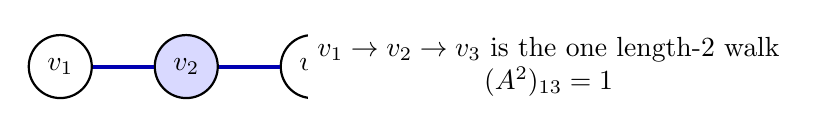
\begin{tikzpicture}[thick,every node/.style={circle,draw,fill=white,minimum size=8mm}]
\node (v1) at (0,0) {$v_1$}; \node[fill=blue!15] (v2) at (1.6,0) {$v_2$}; \node (v3) at (3.2,0) {$v_3$};
\draw[blue!70!black,line width=1.4pt] (v1)--(v2)--(v3);
\node[draw=none,rectangle,align=center] at (6.2,0) {$v_1\to v_2\to v_3$ is the one length-2 walk\\$(A^2)_{13}=1$};
\end{tikzpicture}
\caption{The intermediate vertex $v_2$ contributes one two-edge walk from $v_1$ to $v_3$.}
\end{figure}
\begin{proof}
For $k=1$, the entry $A_{ij}$ is 1 exactly when there is a one-edge walk. Suppose the statement holds for $k$. Then $(A^{k+1})_{ij}=\sum_m(A^k)_{im}A_{mj}$. For each intermediate vertex $v_m$, the product counts walks of length $k$ from $v_i$ to $v_m$ followed by the edge from $v_m$ to $v_j$. Summing over $m$ counts every walk of length $k+1$ exactly once.
\end{proof}

Important: powers count walks, not necessarily paths; walks may revisit vertices and edges. For instance, diagonal entries of $A^2$ count ways to leave a vertex and return in two steps.

\section*{\Enrichment{} Walk counts and linear recurrences}
A sequence $(a_n)$ satisfies a linear recurrence if each later term is a fixed linear combination of earlier terms. Walk counts in a fixed graph often follow such a rule. For the path $P_3$ with vertices $v_1-v_2-v_3$, let $a_n$ be the number of length-$n$ walks from $v_1$ to $v_2$. The first values are
\[
a_0=0,\quad a_1=1,\quad a_2=0,\quad a_3=2,\quad a_4=0,\quad a_5=4,\ldots
\]
Its adjacency matrix satisfies $A^3=2A$, so multiplying by further powers of $A$ shows $A^{n+2}=2A^n$ for $n\geq 1$. Therefore these walk counts obey $a_{n+2}=2a_n$ for $n\geq 1$. The recurrence describes the sequence without listing every walk.

\textbf{Explore.} Verify $A^3=2A$ for $P_3$, then use the recurrence to find the number of length-9 walks from $v_1$ to $v_2$. Does the alternating pattern of zero and nonzero terms make sense from the graph?

\section*{Exercises}
\begin{enumerate}
\item Write the adjacency matrix of the path $v_1-v_2-v_3$.
\item In that graph, explain why $(A^2)_{11}=1$ even though there is no path of length 2 from $v_1$ back to itself under our no-repeated-vertices definition of a path.
\item What does the sum of row $i$ of $A$ equal?
\end{enumerate}
